In 2001, the first analyses of the draft human genome were published in sister papers in \textit{Nature} and \textit{Science}. The Human Genome Project had been budgeted US\$$3$~billion in 1990; by 2020 the cost of sequencing a human genome had dropped to US\$$1,000$, and a relative paucity of data had given way to abundance\citep{gibbs_human_2020}. Biobanks with data from tens or hundreds of thousands of individuals are becoming commonplace.

Every genome carries both the stories of its ancestors and the basic programming of its bearer's physiology. By identifying patterns across many genomes and their associated data, we can infer their histories and study distributions of biomedical traits. The complexities of human history and society, to say nothing of the complexities of biology itself, ensure that this is a non-trivial task.

With each genome spanning $3$~billion base pairs, any mathematical investigation is high-dimensional. Within these data, there are patterns: population structure. It is first necessary to reduce the dimensionality of the data, especially when the goal is visualization. Uniform manifold approximation and projection (UMAP) is a recently-developed method of dimensionality reduction that is rooted in topology---the branch of mathematics dedicated to the study of geometric objects. This thesis explores topological data analysis of population genetics data through UMAP and associated clustering algorithms. We will study how the high-dimensional topology of population genetic data reflects the demographic histories of the individuals we have sequenced, informs us of their biomedical traits, and how to explore this new trove of data.

The thesis is organized into three parts: the introduction with literature review and description of relevant methods; the original contributions to the field; and the final conclusions. The original contributions consist of three chapters that have been previously published as stand-alone manuscripts. In \hyperref[chap:chapter1]{Chapter~2} we apply UMAP to human genetic data for the first time. We use genotype data from three biobanks, generate visualizations and observe patterns in relatedness, demographic histories, geographic distribution, phenotype distributions, and other phenomena. In \hyperref[chap:chapter2]{Chapter~3} we review the applications of UMAP in other human genetic datasets, such as different biobanks or other types of genetic data (e.g. structural variants). Finally, in \hyperref[chap:chapter3]{Chapter~4} we formalize a methodology to use UMAP in higher dimensions ($n \ge 3$), extract clusters algorithmically, and apply these abstractions to a variety of problems common in biobank research.

\section{Genetic diversity}

The human genome spans over $3$~billion nucleobase pairs organized across $23$ pairs of chromosomes---$22$ pairs of autosomes and one pair of sex chromosomes---with some DNA present in mitochondria (mtDNA). The human genome is diploid with one set of chromosomes coming from each parent via their gametes; these chromosomes are created through the process of meiotic recombination, in which the chromosomes of grandparents are aligned, cross over, and recombine. Along with mutation, recombination generates diversity. Approximately $99.9\%$ of DNA shared between humans is identical, with genetic variants (alleles) arising through mutations. Single nucleotide polymorphisms (SNPs) are relatively common variants, usually defined as having a frequency above $1\%$.

Variants that lie along the same chromosome and are not broken up through recombination are co-inherited and are linked. The block of allelic states along a DNA molecule is referred to as a haplotype, and when the same variants exist between two individuals, they are said to be identical by state (IBS). If the shared variant is inherited from a common ancestor without recombination, they are also said to be identical by descent (IBD); alleles that are IBS are typically IBD, with rare exceptions. Alleles that are physically closer are more likely to be inherited together, and those that appear together more often than expected at random are said to be in linkage disequilibrium (LD). Combining two haplotypes gives a diploid genotype, and assuming free recombination, the theoretical maximum number of possible unique haplotypes is $2^L$, where $L$ is the number of SNPs.

Recombination is not uniformly random. DNA that does not lie in the pseudoautosomal regions (PAR1 and PAR2) of the Y chromosome, as well as mtDNA, does not recombine\citep{jobling_human_2013}. Recombination rates also vary within chromosomes with certain regions known to be hotspots\citep{altemose_map_2017}. Germline mutations may result from copying errors during replication or from spontaneous errors from DNA’s instability or external factors like UV radiation. Whole genome sequencing pedigree-based studies estimate the overall mutation rate at about $10^{-8}$ per base pair per generation, though this rate may vary depending on the mechanistic source of the mutation\citep{segurel_determinants_2014}.

\subsection{Population structure}

The distribution of genetic variation is not fully random---genetic differentiation in subpopulations is nearly ubiquitous across organisms. Allele frequencies are influenced by factors like natural selection favouring certain genotypes, founder effects, genetic drift, etc.\citep{hartl2007principles_6}. The mating range of an individual is usually much more constrained than the range of whole species; this leads to isolation by distance (IBD) where there is local structure because of random drift\citep{wright_isolation_1943}. Positive assortative mating, in which individuals choose mates with similar phenotypes, can increase homozygosity\citep{hartl2007principles_6}. Structure may also arise from population bottlenecks or geographic isolation\citep{crow_kimura_1970_3} or admixture between groups that had been separated\citep{crow_kimura_1970_9}. 

Population structure in humans is universal, complex, and multifactorial, resulting from all of the aforementioned causes, and presents as both continuous and discrete\citep{peter_geometric_2022}. Some phenomena unique to humans, such as language\citep{barbujani_zones_1990}, culture\citep{campbell_evolution_2010}, or assortative mating on (e.g.) educational attainment\citep{robinson_genetic_2017} also contribute to population structure. Inferring deep population structure is challenging because of a lack of data and fossil records and the complexity of the required models. Most present-day population structure is relatively recent, having arisen within the last $100,000$ years; prior structure may be best explained by repeated divergence, isolation, and merger between weakly-differentiated \textit{Homo sapiens} populations, though some combination of multiple populations and archaic introgression is also possible\citep{ragsdale_weakly_2023}.

\subsubsection{Hardy-Weinberg principle}

The Hardy-Weinberg model was outlined in 1908. It is used to model genotype frequencies, given several simplifying assumptions\citep{hartl2007principles_2}. If we have a diploid genome with alleles $A_{1}$ and $A_{2}$ that occur at respective frequencies $p$ and $q$, they follow the binomial distribution and are expected to naturally occur at rates
\begin{spacing}{1}
\begin{align*} 
A_{1} \times A_{1} &= p^{2}\\
A_{2} \times A_{2} &= q^{2}\\
A_{1} \times A_{2} &= 2pq
\end{align*} 
\end{spacing}

We can test for excess departure from Hardy-Weinberg equilibrium with a $\chi^2$ statistic, which can indicate technical errors, non-random mating, or population stratification.

\subsubsection{Fixation index}

We expect the level of heterozygosity ($\pi$) to be lower in the presence of population structure. The fixation index ($F_{ST}$) measures population structure; values close to $0$ indicate no structure, while values close to $1$ indicate fully structure populations. Several different estimators exist, depending on the context\citep{bhatia_estimating_2013}. The sample size-independent definition for two populations is:

$$ F_{ST} = \frac{Var(\pi_{i})}{\pi(1-\pi)} $$

where $Var(\pi)$ is the variance in allele frequencies between two populations.

$F_{ST}$ is used as a measure of differentiation between populations. Though it is sometimes described as a pairwise distance between populations, it is not a true mathematical distance as it does not satisfy the triangle equality\citep{arbisser_fst_2020}.

\subsubsection{Wright-Fisher model}

The Wright-Fisher model is a forward simulation of random genetic drift\citep{hartl2007principles_3}. It assumes a fixed population size of $N$ and discrete non-overlapping generations, where individuals from generation $k+1$ draw their alleles at random from generation $k$. It is a simple foundational approach that can be modified to allow for forces like selection, mutation, etc. The alleles follow a binomial distribution with parameters $2N$ and $p$, where $p$ is the proportion of individuals with an allele in the previous generation.

\subsubsection{Coalescent}

The trajectory of $N$ loci can be modelled backwards using the coalescent approach\citep{hartl2007principles_3}. For large N, the probability that two branches coalesce at time t is exponentially distributed with mean N. To incorporate recombination, the problem is formulated as an Ancestral Recombination Graph (ARG) where nodes in the tree are events (either common ancestors or recombinations). This approach scaled poorly, leading to the development of the sequentially Markov coalescent (SMC) approximation where observed data are dependent on underlying sequence data and are modelled as a hidden Markov Model (HMM). There have been considerable improvements in computational approaches for coalescent models and it is an active area of research\citep{kelleher2019inferring}\citep{yc2022evaluation}\citep{zhang2023biobank}.

\subsection{Genome-wide association studies and polygenic scores}

One of the greatest promises of the genomic age is to reveal the genetic architecture of phenotypes and disease risk. Two common and related methodologies are the genome-wide association study (GWAS) and the polygenic score (PGS), also called the polygenic risk score (PRS) when used in the context of disease risk.

The most basic GWAS is a linear regression model. We assume that for some phenotype $y$, the variant $x$ has an additive effect that can be modelled linearly. Then, we can study the association of each variant across the genome, hence the name GWAS. The basic outline is:

$$ y = \beta_0 + x_{j}\beta_{j} + \epsilon \text{ , } \epsilon \sim N(0,\sigma^{2})  $$

where $x_{j}$ is the vector of genotype values at SNP $j$ and $\beta_{j}$ is its effect size. GWAS commonly include terms for genetic relatedness between samples as well as covariates related to genetic ancestry and environment. The model can be written as, e.g.\citep{uffelmann_genome-wide_2021}:

\begin{spacing}{1}
\begin{align*} 
y & = W\alpha + x_{j}\beta_{j} + g + \epsilon \\
g & \sim N(0,\sigma^{2}_{A}\psi) \\
\epsilon & \sim N(0,\sigma^{2}_{\epsilon}I)
\end{align*} 
\end{spacing}

Here, $W$ is the matrix of covariates with associated estimates $\alpha$, $x_{j}$ is a vector of genotypes effect size $\beta_{j}$, $g$ is the random polygenic effect of other SNPs with $\sigma^{2}_{A}$ measuring the phenotype's additive genetic variance and $\psi$ the genetic relatedness matrix, and $\epsilon$ is the regression model residual. To account for multiple testing, the threshold for statistical significance for $\beta_{j}$ is usually set to $10^{-8}$. A variety of methods have been developed to estimate $\beta$ in different frameworks, e.g. via linear mixed-models\citep{loh_mixed-model_2018}, incorporating rare variants\citep{zhou_saige-gene_2022}, using ridge regression\citep{mbatchou_computationally_2021}, etc.

Given a set of estimates $\hat{\beta}$ for each SNP (or each significant SNP), one could construct an estimate of a phenotype as the sum of the estimated effects. For an individual $i$ and for SNPs $j = 1, \dots, p$ we estimate the PGS $y_{i} = \sum_{j}^{p}x_{ij}\hat{\beta_{j}}$. Importantly, PGS have been noted to transfer poorly to populations that are more differentiated from the populations used to estimate the values of $\hat{\beta}$\citep{wang_theoretical_2020}.

Despite significant advances in data collection and methodology, population structure is a persistent confounder in GWAS and PGS. If a variant is more common in one population than another, and a measure differs systematically between them for non-genetic reasons (e.g. environmental exposure, cultural differences in diet, etc.), a GWAS would return a spurious correlation\citep{price_principal_2006}. These systematic differences can accrue in downstream applications like PGS\citep{zaidi_demographic_2020}. 

The effects of structure can be pernicious---in 2019 several studies that had found strong selection signals for height were found to likely be the result of structure\citep{berg_reduced_2019}. Even in populations considered to be relatively homogeneous, structure conferred its bias to PGS estimates\citep{kerminen_geographic_2019}. With applications like PGS becoming more common, understanding population structure in biobanks is critical\citep{kaplan_polygenic_2022}.

\section{Biobanks}

Biobanks are repositories of biological data; we are concerned with those containing genetic data from humans. Large-scale biobanks are now common, with many having data from hundreds of thousands of participants. The Global Biobank Meta-analysis Initiative (GBMI) lists $23$ biobanks with genetic and phenotypic data from over $2.2$ million individuals in total\citep{zhou_global_2022}. These biobanks are commonly used for studying genetic ancestry, demographic history, and biomedical research such as GWAS and PGS.

The sampling methodologies of biobanks vary widely. The 1000 Genomes Project (1KGP)\citep{global_2015} was designed to evenly sample a diverse representation of populations from around the world. Consequently, its population structure closely (but not fully!) aligns with its sampling structure. We study its population structure throughout this thesis, finding previously undetected clusters of structure in \hyperref[chap:chapter1]{Chapter~2}, explore the concept of connectivity in \hyperref[chap:chapter2]{Chapter~3}, and automatically extract clusters in \hyperref[chap:chapter3]{Chapter~4}. As the data are publicly available, there are repositories of our code and data provided for each chapter.

Public health biobanks are commonly sampled from some combination of political jurisdiction and existing health care services. The UK biobank (UKB) and CARTaGENE (CaG), for example, recruit volunteers who are registered with their respective health care administrations within certain geographical regions and political boundaries\citep{sudlow_uk_2015}\citep{awadalla_cohort_2013}. Such administrative records are convenient sampling frames, since they tend to have contact information, associated data such as electronic health records, and established epidemiological methodologies. The wealth of health data, particularly longitudinal data, makes these biobanks invaluable for health care research. 

Their population structure, however, is extraordinarily complex and not known in advance. Even limiting a biobank to one city requires in-depth knowledge of its regional history, its migrations, its cultures, its physical and social environments, etc. Without a means to understand population structure and how it relates to the aforementioned, biobanks can transform from a panacea into a witch's brew of statistical biases. In \hyperref[chap:chapter1]{Chapter~2} and \hyperref[chap:chapter3]{Chapter~4}, we study the relationships between population structure and these variables.

%There are many layers of bias [make a figure here?]

%The combination of 

%\citep{alten_reweighting_2022})


%sex-differential participation bias in 23andme data \citep{pirastu_genetic_2021}

% Casting a wide net creates rich databases that can be combined with established epidemiology methodology (e.g. from previous studies of the populations), but 

%Biobanks are regularly used for studies of demographic history, genetic ancestry, GWAS, and PGS. 

%Their population structure, however, is often enormously complex. Many biobanks are based off of medical cohorts, regional jurisdiction, or volunteer-driven databases for genetic genealogy. Though every biobank is a rich resource, it arrives with its own pitfalls from its sampling methodology.

%The results of biobank studies (e.g. GWAS, PRS) are applied to populations, but how these populations are defined is arbitrary and, arguably, archaic. We can use variables like country of birth or ethnic group, but these are not formally related to genetics and, at best, are proxies. Admixed populations are not well represented---PCA coordinates are themselves a proxy for population structure as it related to a phenotype's distribution.

% Maybe mention in disco?
%Consumer genetic ancestry databases, such as AncestryDNA and 23andMe, contain tens of millions of records, but are fully volunteer-based\citep{mathieson_what_2020}. Though their sample sizes are massive, there is undoubtedly significant selection bias, and the population structure cannot be known in advance.

%23andMe is using UMAP for reference panels\citep{oconnell_population}

% unsupervised learning?

% clustering in popgen?

%\subsection{HDBSCAN(\texorpdfstring{$\hat{\epsilon}$}{f})}
% the {f} here doesn't do anything, but we need a text character for compilation

\subsection{Data sources}

We make use of four biobanks in this research.

\subsubsection{The 1000 Genomes Project}

The 1000 Genomes Project (1KGP) is a publicly available data set of genetic data sampled from many populations from around the world\citep{global_2015}. We used $3,450$ genotypes from the Affy 6.0 platform sampled from $26$  populations. The populations sizes are roughly similar, with between $104$ to $183$ in each group.

\subsubsection{CARTaGENE}

CARTaGENE (CaG) is a cohort of residents of Qu\'{e}bec with genotype data for $29,337$ participants, who were recruited using registration data from the R\'{e}gie de l’assurance maladie du Qu\'{e}bec (RAMQ), the provincial health authority\citep{awadalla_cohort_2013}. In addition to genetic data, it contains questionnaire health data and demographic information such as country of birth and ethnicity.

\subsubsection{Health and Retirement Study}

The Health and Retirement Study (HRS) is a cohort of retired American individuals\citep{juster_overview_1995}. We used genotype data from 12,454 individuals from the Health and Retirement Study (HRS), genotyped on the Illumina Human Omni 2.5M platform. The database contains basic demographic data such as age, US Census Bureau region of birth, and race.

\subsubsection{UK biobank}

The UK biobank (UKB) is a cohort of individuals living in the United Kingdom who were recruited by inviting those registered with the National Health Service (NHS)\citep{sudlow_uk_2015}. It contains the genotypes from $488,377$ participants as well as detailed health data, phenotypic measures, geographic coordinates, and sociodemographic information such as ethnic background.

\section{Exploratory data analysis}

Traditional statistical analyses of biological data follow the recommendations of R.A. Fisher in the 1930s\citep{holmes_modern_2019}. They have a linear structure: beginning with a biological question, an investigator forms a hypothesis and an associated null ($H_0$), designs an experiment, collects data, tests $H_0$ with a p-value, and formulates a conclusion. Beginning in the 1970s, statistician John W. Tukey proposed the alternative framework of exploratory data analysis (EDA)\citep{tukey_1977,hoaglin_john_2003}. This approach is iterative and instead begins with the data: we visualize it, understand it, and use it to inform what sort of analysis to use in an accompanying confirmatory data analysis. The two contrasting approaches are schematized in Figure~\ref{fig:paradigms}.

\begin{figure}[ht!]
\centering
\begin{subfigure}{0.3\textwidth}
    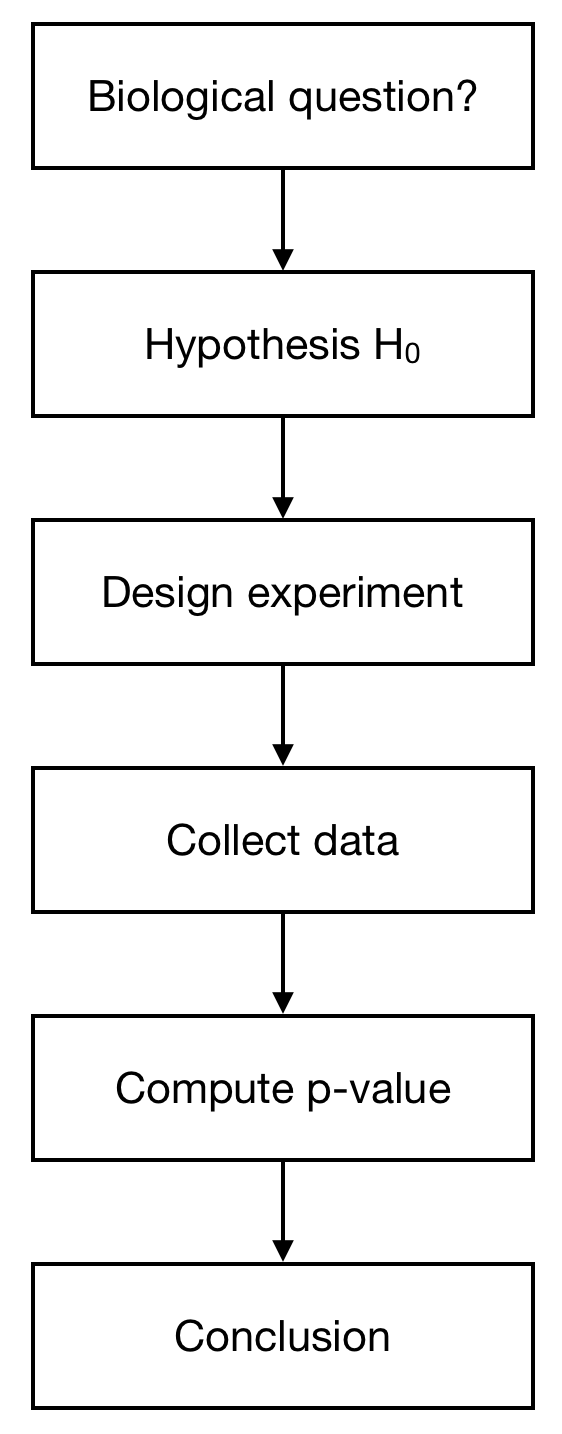
\includegraphics[height=0.5\textheight]{main_figures/intro/fisher_paradigm.png}
    \caption{Fisher's paradigm.}
    \label{fig:fisher}
\end{subfigure}
\hfill
\begin{subfigure}{0.65\textwidth}
    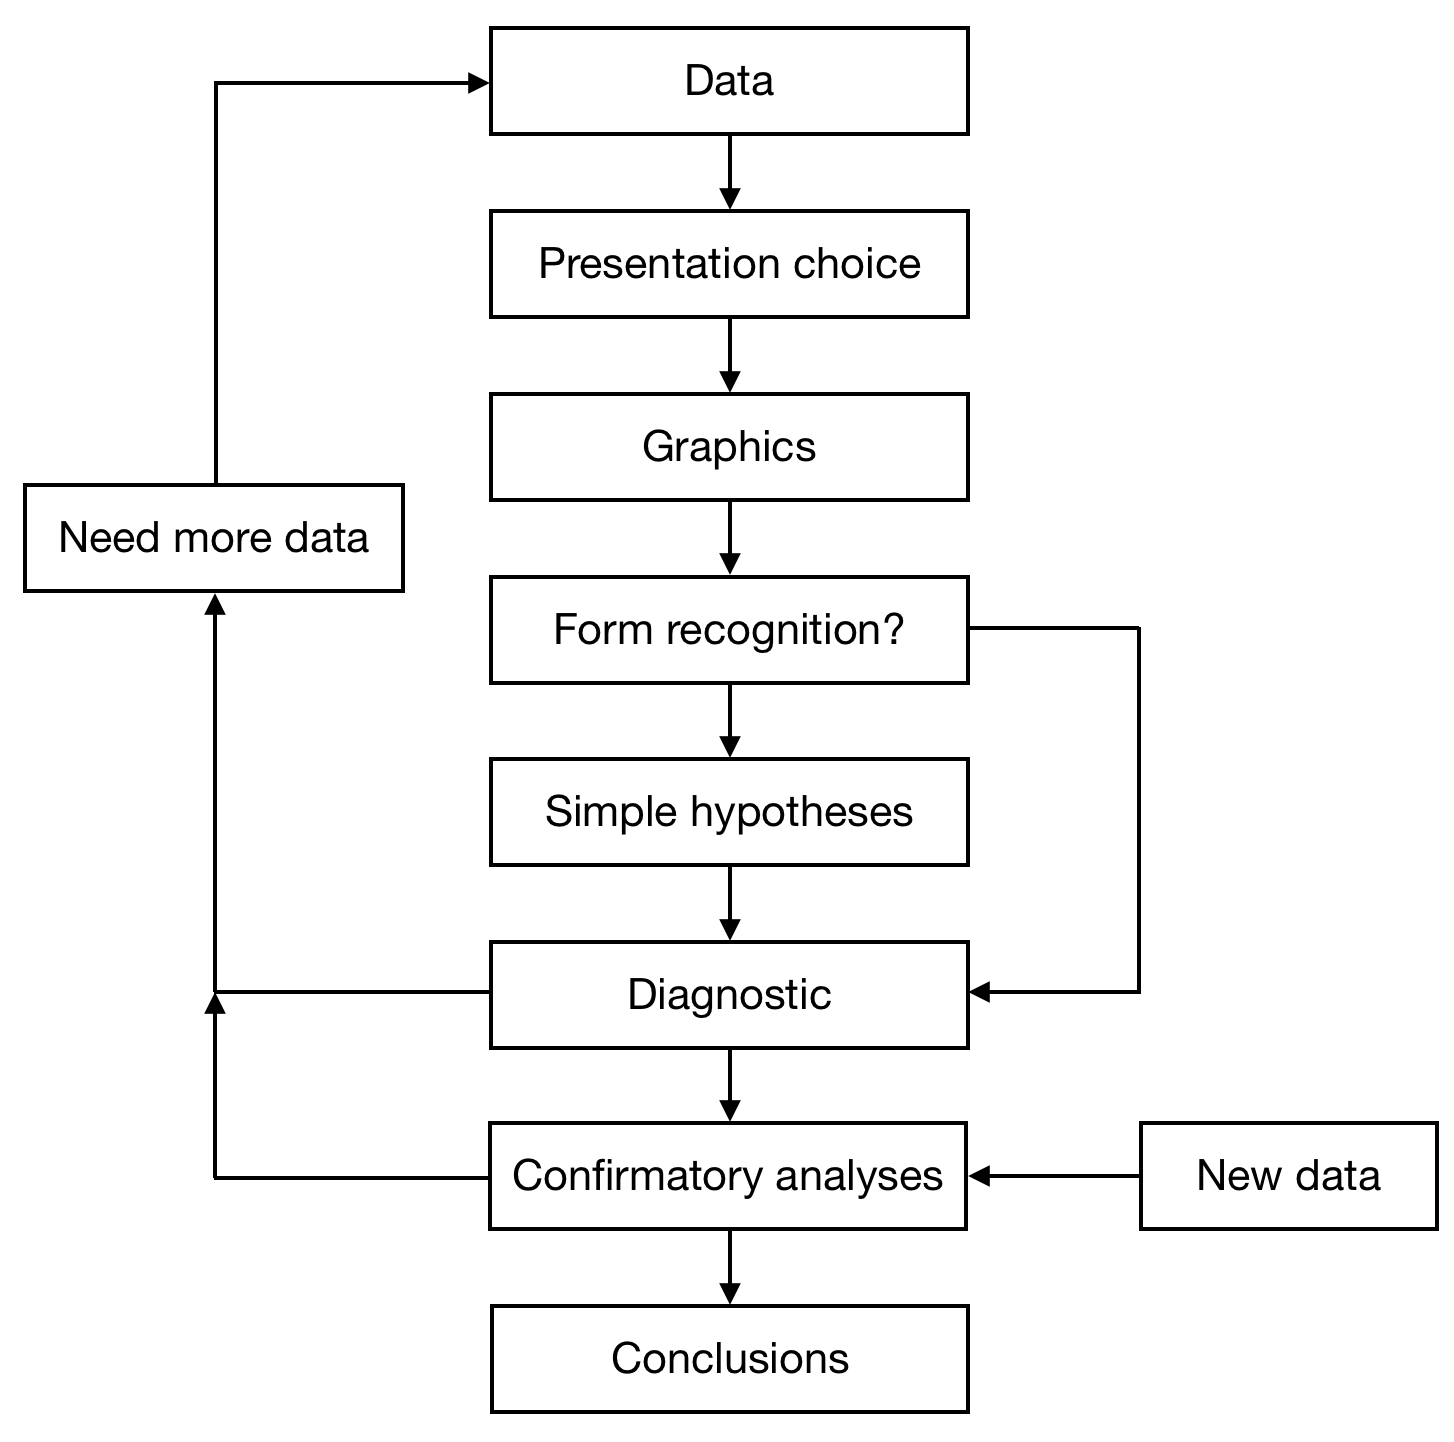
\includegraphics[height=0.5\textheight]{main_figures/intro/tukey_paradigm.png}
    \caption{Tukey's paradigm.}
    \label{fig:tukey}
\end{subfigure}
\caption[Contrasting Fisher's paradigm with Tukey's paradigm in biology]{\textbf{Contrasting Fisher's paradigm with Tukey's paradigm in biology.} Fisher's paradigm (left) takes a sequential approach to data analysis, beginning with a well-defined question and strong assumptions. Tukey's paradigm (right) is iterative, beginning with the data, emphasizing exploratory analysis through visualization, and complemented by confirmatory analyses that are robust and do not rely on complex assumptions\citep{holmes_modern_2019}.}
\label{fig:paradigms}
\end{figure}

Writing in 1980, Tukey emphasized that science neither begins with a tidy question nor ends with a tidy answer\citep{tukey_we_1980}. This is especially true in modern biology. Statistical questions from the 1930s typically had a few parameters $p$ with a manageable sample size $N$ (where $N > p$), and the people posing questions were involved in data collection. Today we sit at the opposite extreme; it is not unusual for data to have $p >> N$ with the two values differing by orders of magnitude. When studying a biobank, we may have several thousand individuals and several hundred thousand genetic markers. Generally, the people investigating data have not collected it. These factors make Tukey's paradigm much better suited to our analytical needs\citep{holmes_modern_2019}. 

\subsection{Dimensionality reduction}

In Figure~\ref{fig:tukey}, the iterative process includes presentation choices, graphics, and form recognition. This provokes a natural question: what approaches ought we use here? With genomic data comes the ``curse of dimensionality'': though we have many dimensions to our data, the signal is sparse and many methods are computationally intractable. This motivates dimensionality reduction---we wish to reduce our data to a relatively low number of dimensions, ideally preserving important characteristics of the data. Given a satisfactory representation of the data set, we can visualize it.

\subsubsection{Principal component analysis}

Principal components analysis (PCA) is a non-parametric linear transformation that projects data onto a series of orthogonal axes based on a linear combination of the original data. The axes are generated and ordered according to their eigenvalues, and the ratio of each axis' corresponding eigenvalue to the sum of all eigenvalues represents the variance explained by that axis. PCA fits an ellipsoid around the data in high dimensions and the axes of that ellipsoid are the principal components. By only selecting the largest axes---corresponding to the most explained variance --- we can reduce the dimensionality of our data while preserving significant explanatory value. We can also interpret our dimensionally reduced data in terms of how much of the overall variance it explains. Principal components are calculated through eigendecomposition of the covariance matrix; a derivation for genotype data is given in \hyperref[appendix:AppendixA]{Appendix~A}. A detailed examination of PCA in the context of population genetics can be found in \citep{mcvean_genealogical_2009}. 

PCA has seen wide application in population genetics. The top PCs often reflect isolation-by-distance and are used for visualization (e.g. within Europe\citep{novembre2008europe}). However, using them for visualization requires selecting which components to examine and is limited to $2$ or $3$ dimensions; if there is signal beyond the first few PCs, it may go unnoticed. We expand on this in \hyperref[chap:chapter1]{Chapter~2}.

They are also used to correct for population structure in genome-wide association studies (GWAS) by their inclusion as covariates in models\cite{price_principal_2006}. There are varying rules-of-thumb on how many PCs to include in a model, such as using the top $10$, looking for an ``elbow'' in the scree plot, or testing for eigenvalue significance in the Wishart distribution; however, these are merely conventions. We explore the impact of PC adjustment for phenotypes in biobanks in \hyperref[chap:chapter3]{Chapter~4}. 

\subsection{Topological data analysis}

% Note to self: Rewrite this in terms of popgen challenges
% can maybe get philosophical here
We are often interested in learning about our data in to understand its large-scale structure, e.g., identifying different cell types or related individuals. Though we have some definitions of distances, we are interested in notions of \textit{similarity}, \textit{nearness}, and \textit{connectivity}. Topology provides the mathematical machinery for ideas rooted in qualitative geometry\citep{carlsson_topology_2009}. Topological data analysis (TDA) is a set of statistical methods that uses ideas of shape and connectivity to study data\citep{wasserman_topological_2018}. We will focus on applications of manifold learning, nonlinear dimensionality reduction, and density clustering.

TDA assumes that we observe a sample $X_1, \dots, X_n \sim P$ with $P$ supported on some set $\supp(P) = \mathcal{X} \subseteq \mathbb{R}^d$. 
In the simplest case of manifold learning, we suppose that $P$ is actually supported on some set $S$ with dimension $r$, where $r < d$ and $S$ is a smooth and compact manifold, and we may estimate $S$. PCA is a special case of linear manifold learning where data are assumed to lie on or near an affine subspace\citep{wasserman_topological_2018}. In cases where there is local nonlinear structure (such as clustering), nonlinear methods of manifold learning are more useful\cite{izenman_introduction_2012}.

\subsection{\texorpdfstring{$\mathbf{t}$}{f}-distributed stochastic neighbour embedding}
% the {f} here doesn't do anything, but we need a text character for compilation

$t$-distributed stochastic neighbour embedding ($t$-SNE) is a method of manifold learning used for visualization that was developed in 2008\citep{maaten_visualizing_2008}. By then, several methods existed to approximate the local structure of manifolds, but they suffered from the ``crowding problem''---in an attempt to preserve local distances between points, many of them are crunched together, eliminating the gaps between clusters. $t$-SNE addressed this by introducing a repulsion force between points, modelling pairwise distances between points $i$ and $j$ as a $t$-distributed random variable with $1$ degree of freedom (equivalent to a Cauchy distribution). The distances are modelled as probabilities:

$$q_{ij} = \frac{(1 + ||y_{i} - y_{j}||^{2})^{-1}}{\sum_{k \neq l}(1 + ||y_{k} - y_{l}||^{2})^{-1}}$$

This choice was largely ad-hoc and was later found to work because it optimized structure at the local scale (i.e. within clusters) as well as causing points to repel each other (i.e. causing clusters to separate)\citep{carreira-perpinan_elastic_2010}. This repulsion allowed $t$-SNE and related methods to preserve topology\citep{wasserman_topological_2018}. Because $t$-SNE can only reduce data to $2$ or $3$ dimensions, it was not recommended as a general purpose dimensionality reduction algorithm\citep{maaten_visualizing_2008}. It saw considerable use in visualization in single-cell genomics\citep{kobak_art_2019}, but its application in population genetics was limited (e.g. \citep{li_application_2017}). We provide details on $t$-SNE's performance in population genetics in \hyperref[chap:chapter1]{Chapter~2}.

\subsection{Uniform manifold approximation and projection}

Uniform manifold approximation and projection (UMAP) is a general purpose dimensionality reduction method rooted in algebraic topology and Riemannian geometry that was introduced in 2018\citep{mcinnes_umap_2020}. Unlike the more heuristic approach of $t$-SNE, the motivation behind UMAP is to represent the high-dimensional topology of data in low dimensional space. We will briefly outline the intuition underlying UMAP; details on the topology and theoretical justifications are available in \citep{mcinnes_umap_2020}, with a more applied explanation available in online documentation\citep{mcinnes_umapdoc_2018}.

We assume our data $X = \{X_{1}, \dots, X_{n}\}$ lay on some manifold and are uniformly distributed. For this assumption to hold, each point $X_{i}$ has its own custom distance, defined as the normalized distance to its $k\textsuperscript{th}$ nearest neighbour; thus, each $X_{i}$ has its own metric space, and is the centre of a unit ball that extends to the $k\textsuperscript{th}$ nearest neighbour. If we represent this as a graph, each $X_i$ is a point with edges to its $k$ neighbours, where the distances represent the edge weights. If we represent this as a simplicial complex, a point is a $0$-simplex and an edge is a $1$-simplex; according to theory, this simplicial complex forms an open cover of the underlying topological space. As the edge weights are between $0$ and $1$, we may also interpret the values as the belongingness to an open cover rather than a binary ``yes'' or ``no'' value---a fuzzy topological cover. To harmonize the respective edge weights $a, b$ from points $X_{a}$ to $X_{b}$ (since each point has its own local metric), UMAP defines the combined weight as $a + b - a \times b$, interpreted as the probability that an edge weight between $X_{a}$ and $X_{b}$ exists. The final high-dimensional product is a fuzzy simplicial complex, which can be represented as a weighted graph, and is a fuzzy topological representation of the data.

For the low-dimensional representation, we carry out the same process of building a fuzzy topological representation. However, rather than using a locally-varying metric, we assume that our data will lay on a low-dimensional Euclidean space, and we specify a minimum distance we wish to have between our points in this space. The algorithm then minimizes the cross-entropy function between the high- and low-dimensional representations. If $E$ is the set of all possible $1$-simplices, $w_{h}(e)$ is the weight of edge $e$ in the high-dimensional space and $w_{l}(e)$ the low-dimensional space, we minimize:

$$ \sum_{e \in E} w_{h}(e) \log{\left(\frac{w_{h}(e)}{w_{l}(e)}\right)} + (1 - w_{h}(e)) \log{\left(\frac{1 - w_{h}(e)}{1 - w_{l}(e)}\right)} $$

This mathematical machinery allows for reduction of data to an arbitrary number of dimensions and for topological interpretations. The value of $k$ defines the scale of the topology we wish to approximate, with lower values being more local and finer-scale and higher values approximating broader manifold structure. Each chapter of this thesis discusses the uses and parametrizations of UMAP in population genetics: briefly, lower values of $k$ approximate closer relationships, e.g., at a structure as fine-scale as families; higher values of minimum distance facilitate visualization, while lower values facilitate algorithmic cluster detection. Points that appear near each other in low-dimensional space are closely related to one another. UMAP often generates visual clusters---while the clusters themselves can be interpreted, the distances between them are generally not meaningful. Importantly, UMAP is a fast and scalable algorithm, capable of handling millions of data points.

UMAP is the core method of this thesis. In \hyperref[chap:chapter1]{Chapter~2}, we use UMAP in population genetics for the first time, exploring its potential applications thoroughly and compare it to PCA and t-SNE. Having been quickly adopted after our publication, in \hyperref[chap:chapter2]{Chapter~3}, we review its uses in the field and discuss different data inputs and parametrizations. In \hyperref[chap:chapter3]{Chapter~4}, we introduce the use of UMAP for topological stratification of complex biobank data by using it to pre-process data for clustering rather than visualization.

\subsection{Clustering}

Broadly, clustering is a class of methods that puts similar data points into the same cluster while keeping dissimilar data points in different clusters\citep{ben-david_clustering_2018}. Clustering in population genetics can be separated into model-based methods, which are common in global ancestry estimation, and distance-based methods, which measure pairwise distances between individuals. Though we use the former in some analyses, \hyperref[chap:chapter3]{Chapter~4} focuses on the latter, specifically density clustering.

It can be useful to model populations as $K$ discrete demes, e.g. when modelling admixture, studying population splits and merges, or testing the transferability of GWAS and PGS. Clustering is a natural approach to this problem. A variety of clustering methods have been used in population genetics. These methods often require specifying $K$; though multiple methods have been proposed to estimate $K$ (e.g. \citep{evanno_detecting_2005,verity_estimating_2016}), it does not have a ``correct'' value as genetic data does not fall into natural discrete groups\citep{lawson_tutorial_2018}.

\subsubsection{Model-based clustering}

Model-based clustering assumes that observations are randomly drawn from some parametric model. The first such method used in population genetics was STRUCTURE, in 2000, which assumed that each cluster was defined by some allele frequency; having observed the genotypes $X$, it infers the populations of origin $Z$ and allele frequencies $P$ through Bayesian modelling of $Pr(Z, P|X)$\citep{pritchard_inference_2000}. Each genome is then modelled as a mixture of some $K$ source populations---often presented in literature as a stacked bar graph where each individual is one bar with split ancestry proportions---and termed ``global ancestry estimation''\citep{alexander_fast_2009}. The idea has since evolved into many other methods (e.g. ADMIXTURE\citep{alexander_fast_2009}, FRAPPE\citep{tang_estimation_2005}, sparse non-negative matrix factorization\citep{frichot_fast_2014}, archetypal analysis\citep{gimbernat-mayol_archetypal_2022}) and is an active area of research to handle more complex model assumptions and larger data sets.

\subsubsection{Distance-based clustering}

One of the most common distance-based algorithms is $K$-means clustering. Developed in the 1970s, it works by dividing $M$ points in $N$ dimensions into $K$ groups by minimizing the within-cluster sum of squares\citep{hartigan_algorithm_1979}. $K$-means clustering has been used to define populations by, e.g., using the coordinates of individuals in PCA space and comparing to some known reference population within a cluster. $K$-means implicitly assumes that data points form a Gaussian distribution around some centroid\citep{mcinnes_accelerated_2017}. However, genetic data do not naturally present as clouds about some centroid. Data points are either partitioned arbitrarily, stripping clusters of interpretation, or the distances from the centroids have sharp cut-off points. In the latter case many individuals, particularly from admixed populations or uncommon genetic ancestries, will never be placed into a cluster, especially if there is no reference population to compare them to\citep{ding_polygenic_2023}.

\subsubsection{Density clustering}

% this density lambda is set to 1/epsilon

Density clustering finds sets of data with a high density of points; a formal outline can be found in Wasserman's review of TDA\citep{wasserman_topological_2018}. Briefly, assume we observe a sample $X_{1}, \dots , X_{n}$ from some distribution $P$ with density $p$ where $X_{i} \in \mathcal{X} \subseteq \mathbb{R}^d$. For any $\lambda \ge 0$, we define the upper level set $L_{\lambda} = \{x: p(x) > \lambda \}$. The density clusters at level $\lambda$ are denoted by $\mathcal{C}_{\lambda}$ and are the connected components of $L_{\lambda}$. The set of all density clusters is:

$$ \mathcal{C} = \bigcup_{\lambda \ge 0} \mathcal{C}_{\lambda} $$

By varying the threshold $\lambda$, level sets $L_{\lambda}$ become nested within each other; that is, if $A, B \in \mathcal{C}$ then $A \subset B$ or $B \subset A$ or $A \cap B = \emptyset$. Thus the set $\mathcal{C}$ can be represented as a tree, and each branch represents a cluster. This approach is useful if we know there is structure in our data but do not know how many clusters exist---if we can find an appropriate threshold for density, we can discover the structure. Unlike other clustering methods, this approach does not necessarily require specifying a number of clusters $K$ in advance---though some algorithms do incorporate $K$, we do not consider them in this thesis.

The first density clustering algorithm was Density Based Spatial Clustering of Applications with Noise (DBSCAN), developed in 1996\citep{ester1996density} and became the basis of many others\citep{khan_dbscan_2014}. DBSCAN formalized the intuition that clusters were spaces that were dense with data, while areas that were relatively sparse were noise. For each point in a cluster, the neighbourhood of a given radius $\epsilon$ must contains at least $m$ points. Any points that meet this criterion, or fall within the neighbourhood, are assigned to clusters, while the rest are deemed noise. However, this requires a global density $\epsilon$ threshold---clusters of variable densities are not considered. 

A hierarchical version (HDBSCAN) that varied the thresholds $\epsilon$ was developed in 2013\citep{campello_density-based_2013}. It required only the minimum points $m$ and optimized across the tree for $\mathcal{C}$, selecting values of $\epsilon$ that led to the highest stability, and defining $\lambda = \frac{1}{\epsilon}$. Now we are presented with a dilemma: what if our data set is large and contains dense clusters \emph{and} relatively sparse clusters? Using DBSCAN with its global $\epsilon$ threshold would miss small clusters, while using HDBSCAN with a variable $\epsilon$ with a low minimum points $m$ would break large clusters apart into microclusters, and in both cases many points would be discarded as noise. This motivated HDBSCAN($\hat{\epsilon}$), a hybrid version that prevents clusters below a specified density threshold from splitting further, which would allow a better representation of the structure of data\citep{malzer_hybrid_2020}. In addition to $m$, we provide the algorithm with a second parameter $\hat{\epsilon}$, which provides a global minimum density for points to still be considered part of clusters.

This latter method is key to \hyperref[chap:chapter3]{Chapter~4}, where we pre-process biobank data with UMAP and apply HDBSCAN($\hat{\epsilon}$) to extract clusters. The sizes of populations in many biobanks vary widely---it is not unusual for a biobank to have a few ancestrally-related populations making up, e.g., $90\%$ of the cohort with the remaining $10\%$ consisting of several small populations whose genetic ancestries differ from the majority and from each other because of immigration history, admixture, highly-structured demographic history (as in the case of islands), etc. The UKB, for example, has $488,377$ genotyped individuals; well over $90\%$ claim European ancestry, but the remaining groups still number in the thousands.

%Stepping back, this last regime describes modern biobank data well. Dense areas in genetic space are those where many individuals are ``close'' to each other; that is, they have similar distributions of genetic variants, representing a similar demographic history. Biobanks generally do not have evenly-balanced populations, particularly when they are constructed using jurisdiction (e.g. a biobank may recruit participants from a country, province, or metropolitan area). 

%More explicit details on cluster selection are available in \citep{mcinnes_accelerated_2017} and \citep{malzer_hybrid_2020}, with an outline in \hyperref[appendix:AppendixB]{Appendix~B}.

%What does data \emph{truly} look like?

%- we do UMAP to make our data accessible to hdbscan, we use hdbscan because it has properties that are very nice, also it has probabilistic and topological interpretations
%- population structure is basically "similarity" and "nearness"

\section{Rationale and objective of research}

The biobank space is rapidly growing with large and diverse cohorts being announced and released on a regular basis. Methods like GWAS and PGS are now standard and studying genetic ancestry is common both in scientific circles and in consumer-facing products. We require new tractable methodologies that can bolster our understanding of population structure in these data sets, which continue to grow in size and complexity. We also must understand the interplay between genetics, phenotypes, and the environment. 

Thus the main objectives of this thesis are:
\begin{itemize}
\item To apply topological data analysis to human genetic data
\item To use nonlinear dimensionality reduction and density clustering to characterize population structure in a variety of biobanks, focusing on using UMAP and HDBSCAN($\hat{\epsilon}$)
\item To provide a framework for a new methodology for population genetics and will demonstrate its utility to the field
\item To relate population structure to other collected data in biobanks, such as population labels, phenotypic information, geographic coordinates, demographic history, genetic ancestry, and other variables
\item To study the implications of our results to GWAS and PGS
\end{itemize}

\clearpage